\subsection{First Research Question}
\label{sec:ResearchQuestion1}
The first research question of this project states:
\\
"How well can dynamic networks be modelled using a Stepwise Constant Velocity Model (SCVM) representation in Euclidean latent space?"
\\\\
In order to answer this question, the modelling approach will be evaluated on synthetically generated data as well as real dataset 1, using evaluation methods described under section \ref{sec:Method:Evaluation}.


\subsubsection{Single-Step Modelling of Synthetic Data}
\label{sec:ResearchQuestion1:singleStepSynthetic}
The first part of answering research question one consists of confirming proper modelling performance of the SCVM in a single-step scenario.
This is done as to ensure correct performance, and it is evident that if modelling single-step data does not work as intended, multi-step modelling will neither.

For this part, synthetic dataset 1 is utilized, which is synthesized using a single velocity vector, as explained in section \ref{sec:Data:SyntheticData:SyntheticDataset1}.
\\\\
\textbf{Loss and beta convergence results}
\\
To reiterate, the models are trained for 5000 epochs on the full dataset 1 as one training batch with learning rate $\alpha = 0.025$. 
The SCVM, fitting one velocity vector for each node, ie. one step, is compared to a baseline model which has no velocity vector, hence no dynamics. 
Further, for comparison purposes, the ground truth model with true starting positions and velocity of dataset 1 is also utilized in these results.
\\
Below, table \ref{tab:SingleStep1} shows the learned beta parameter and final average negative log likelihood, the average loss over number of dyads, of the aforementioned models.

\begin{table}[H]
\centering
\begin{tabular}{|l|c|cc|}
\hline
Model         & \multicolumn{1}{l|}{Num. Epochs} & Beta & Avg. Loss \\ \hline
Ground Truth  & -                                & 7.5  & -82377.99  \\
No dynamics Baseline & 5000                             & 6.487  & 34715        \\
1 Step SCVM  & 5000                             & 7.495   & -82376.19      \\ \hline
\end{tabular}
\caption{Final learned $\beta$ value and average loss for baseline trained model.}
\label{tab:SingleStep1}
\end{table}
\noindent
Here, the single step SCVM has converged to within $0.005$ of the true beta value, and proves much better than the no dynamics baseline, which is no way near the correct $\beta$.
\\\\
\textbf{Intensity rate comparison results}
\\
The intensity rates for each dyad is seen in figure \ref{fig:RQ1:baseline_intensity} for the no dynamics baseline model:

\begin{figure}[H]
    \centering
    \begin{subfigure}[b]{\textwidth}
        \centering
        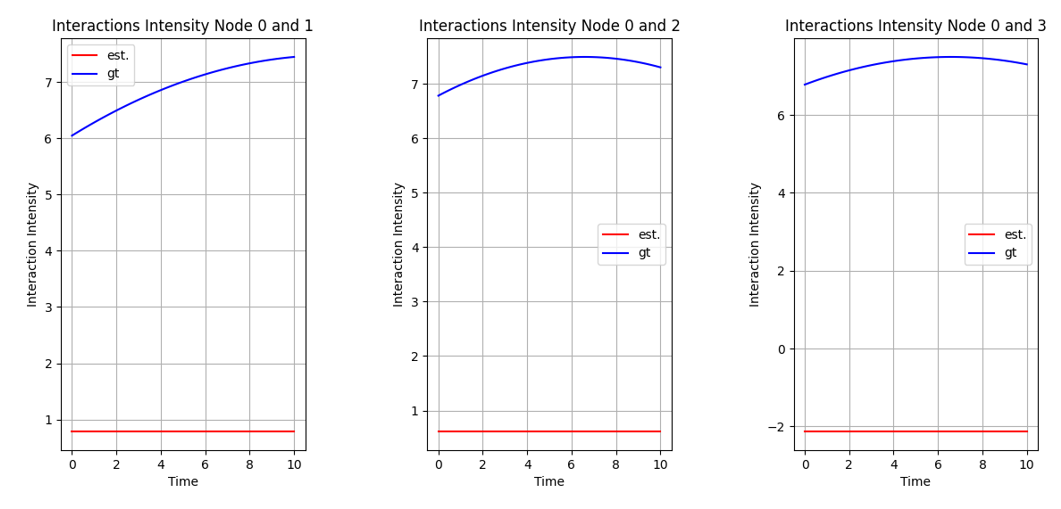
\includegraphics[width=\textwidth]{0_images/rq1_baseline_intensity_plot1.png}
    \end{subfigure}
    \vfill
    \begin{subfigure}[b]{\textwidth}
        \centering
        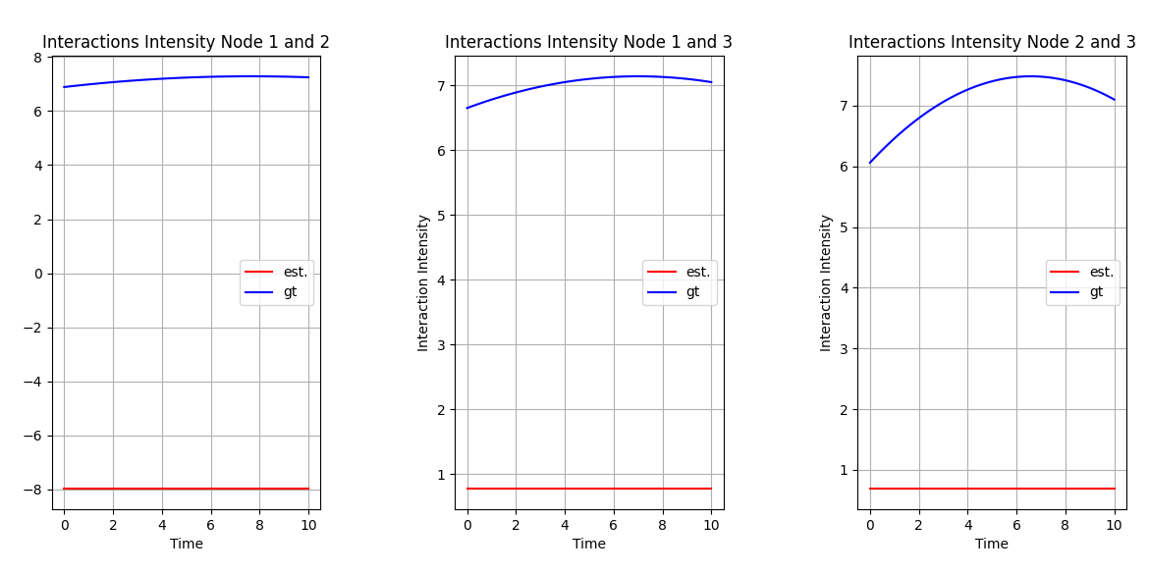
\includegraphics[width=\textwidth]{0_images/rq1_baseline_intensity_plot2.png}
    \end{subfigure}
    \caption{Basline model's node pair interaction intensity for synthetic dataset 1 trained for 5000 epochs. Blue line is the ground truth model, red is the baseline model.}
    \label{fig:RQ1:baseline_intensity}
\end{figure}
\clearpage
\noindent
Intensity rates for the SCVM fitting one step is seen in figure \ref{fig:RQ1:SCVM_intensity}:
\begin{figure}[H]
    \centering
    \begin{subfigure}[b]{\textwidth}
        \centering
        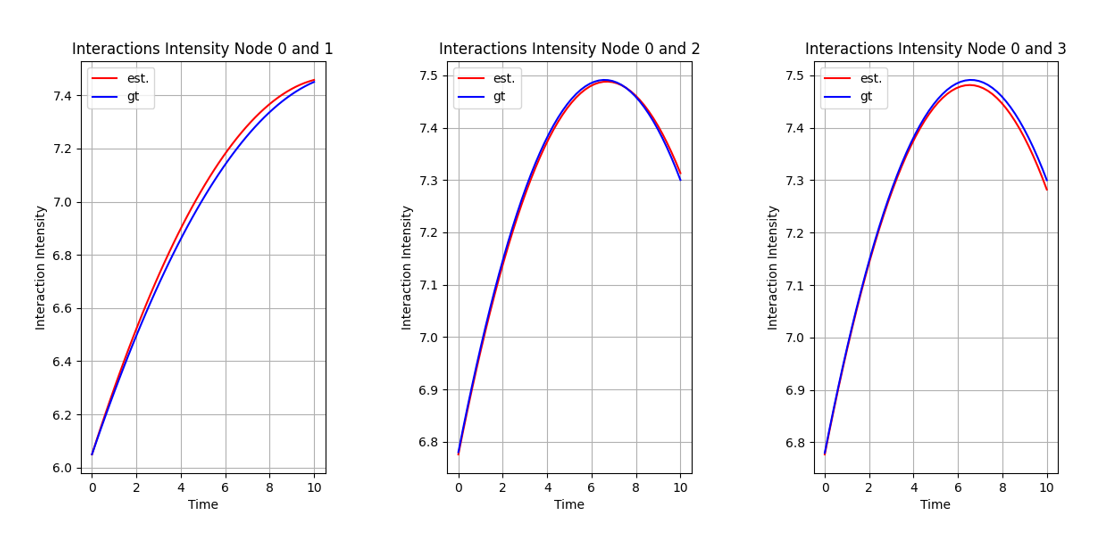
\includegraphics[width=\textwidth]{0_images/rq1_SCVM_intensity_plot1.png}
    \end{subfigure}
    \vfill
    \begin{subfigure}[b]{\textwidth}
        \centering
        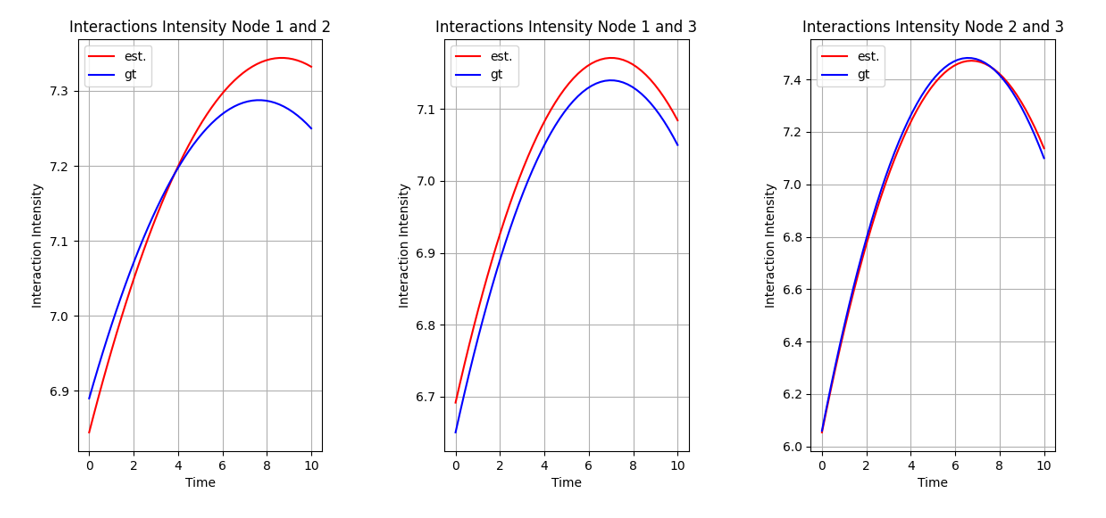
\includegraphics[width=\textwidth]{0_images/rq1_SCVM_intensity_plot2.png}
    \end{subfigure}
    \caption{SCVM model's node pair interaction intensity for synthetic dataset 1 trained for 5000 epochs. Blue line is the ground truth model, red is the one step SCVM.}
    \label{fig:RQ1:SCVM_intensity}
\end{figure}
\noindent
The interaction intensity plots show that the learned parameters of the single step SCVM model the ground truth dataset much better than the no dynamics baseline.
\clearpage
\noindent
\textbf{Interaction removal results.}
\\
The results from interaction removal, as explained in section \ref{sec:Method:Evaluation:AUC}, shows a worse than random accuracy for the no dynamics baseline model, seen in figure \ref{fig:RQ1:baseline_accuracy}.
\begin{figure}[H]
    \centering
    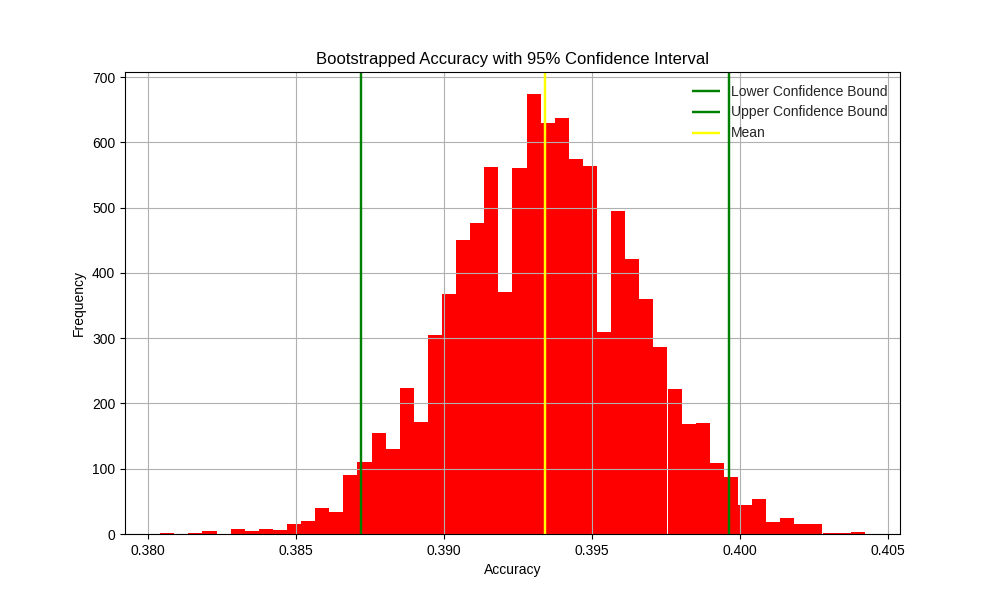
\includegraphics[width=0.8\textwidth]{0_images/rq1_baseline_accuracy.png}
    \caption{Baseline model's interaction removal accuracy with 95 \% confidence interval, for synthetic dataset 1 trained for 5000 epochs.}
    \label{fig:RQ1:baseline_accuracy}
\end{figure}
\noindent 
The single step SCVM has a better, but still low accuracy, for predicting the correct node pair interaction, seen in figure \ref{fig:RQ1:SCVM_accuracy}.
\begin{figure}[H]
    \centering
    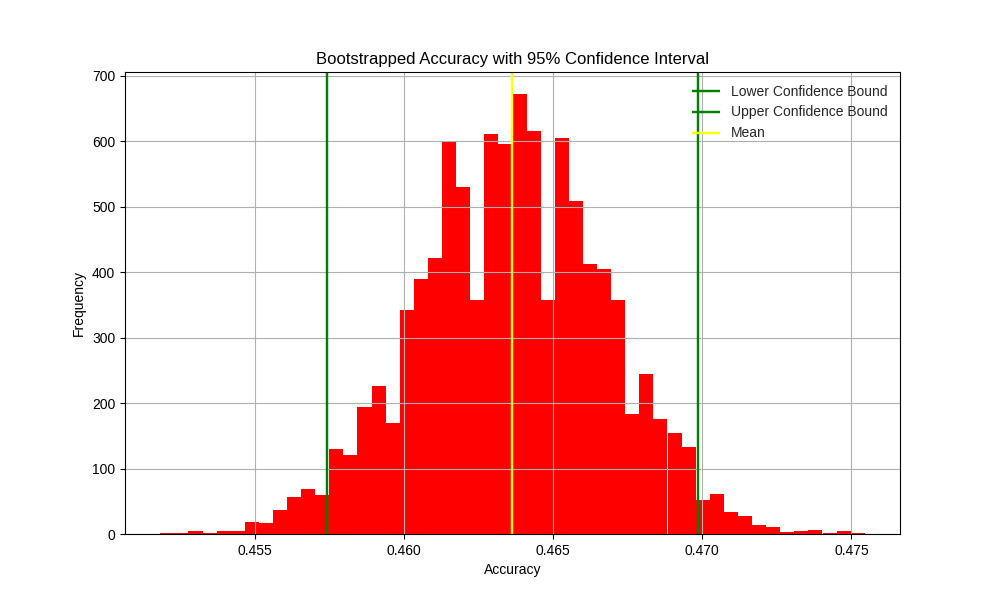
\includegraphics[width=0.8\textwidth]{0_images/rq1_SCVM_accuracy.png}
    \caption{Single step SCVM model's interaction removal accuracy with 95 \% confidence interval for synthetic dataset 1 trained for 5000 epochs.}
    \label{fig:RQ1:SCVM_accuracy}
\end{figure}
\noindent
However, a difference for the SCVM compared to the baseline is that the SCVM actually achieves an accuracy similar to that of the ground truth model, as both  models are within a 46-47 \% accuracy confidence interval in the tests.
The accuracy of the baseline is seen in figure \ref{fig:RQ1:baseline_accuracy}.
\begin{figure}[H]
    \centering
    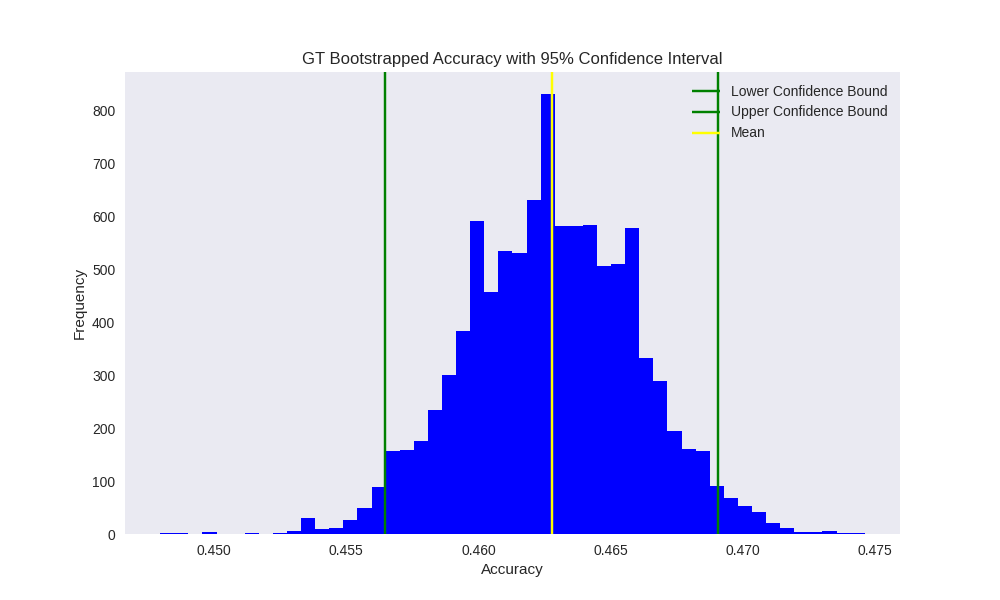
\includegraphics[width=0.8\textwidth]{0_images/rq1_GT_accuracy_SCVM.png}
    \caption{Ground truth model interaction removal accuracy with 95 \% confidence interval for synthetic dataset 1.}
    \label{fig:RQ1:baseline_accuracy}
\end{figure}

\clearpage
\noindent
\textbf{Dyad removal results}
\\
The baseline model with no dynamics is discarded here, as it already proved unable to properly model the dynamics of dataset 1, see figure \ref{fig:RQ1:baseline_intensity}, and removing one dyad from dataset 1 just makes this worse. 
Instead, we look at figure \ref{fig:RQ1:SCVM_dyadremoval} which shows the resulting node interaction intensity plots for the single step SCVM trained on dataset 1 in which all interactions for dyad (0,1) have been removed:
\begin{figure}[H]
    \centering
    \begin{subfigure}[b]{\textwidth}
        \centering
        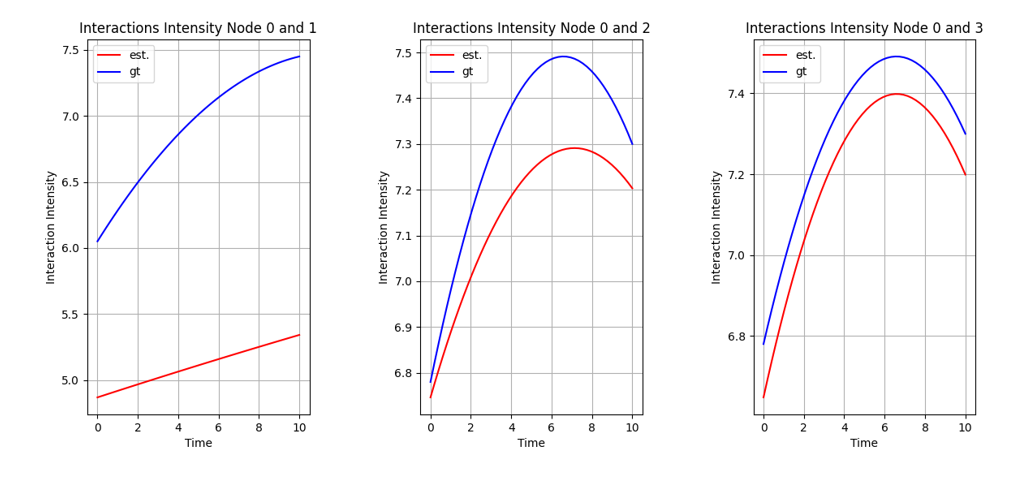
\includegraphics[width=\textwidth]{rq1_dyad_removal_SCVM1.png}
    \end{subfigure}
    \hfill
    \begin{subfigure}[b]{\textwidth}
        \centering
        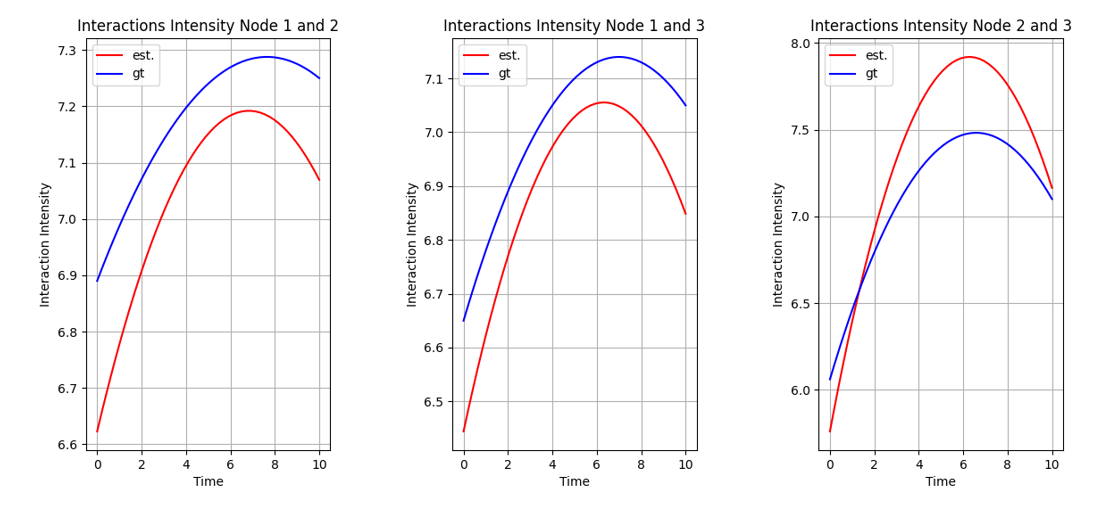
\includegraphics[width=\textwidth]{rq1_dyad_removal_SCVM2.png}
    \end{subfigure}
        \caption{SCVM intensity plot after removing node pair (dyad) (0,1).}
    \label{fig:RQ1:SCVM_dyadremoval}
\end{figure}
\noindent
Above figure shows the clear negative impact removing the data of an entire dyad has.
The model is firstly not capable of inferring the interaction intensities of dyad (0,1) from the interactions of the remaining dyads, as can be seen from the badly estimated intensity plot.
The learned parameters further result in worse fits of the remaining dyads, when compared to the single step SCVM trained on the entire dataset, as seen in figure \ref{fig:RQ1:SCVM_intensity}.




\subsubsection{Multi-Step Modelling of Synthetic Data}
\label{sec:ResearchQuestion1:multiStepSynthetic}
The second part of answering the first research question evaluates the SCVM with 10 steps to test its capabilities when fitting multiple steps and hence multiple velocities for each node. 
The model is compared to the single step SCVM from earlier, and results of the ground truth 10 step model are also provided. 
The test uses the synthetic dataset 2, described under section \ref{sec:Data:SyntheticData:SyntheticDataset2}.
\\\\
\textbf{Loss and beta convergence results}

\begin{table}[H]
\centering
\begin{tabular}{|l|c|cc|}
\hline
Model         & \multicolumn{1}{l|}{Num. Epochs} & Beta & Avg. Loss \\ \hline
Ground Truth  & -                                & 7.5  & -192208.05 \\
1 Step SCVM & 5000                          & 6.971 &  -183478.37      \\
10 Step SCVM & 5000                          & 7.499   & -191501.75      \\ \hline
\end{tabular}
\caption{Learned $\beta$ value and negative log loss for models on synthetic dataset 2 \ref{sec:Data:SyntheticData:SyntheticDataset2}}
\label{tab:MultiStep1}
\end{table}
\noindent 
The convergence results show a clear difference between the single step fitted SCVM, and the 10 step fitted SCVM, where the latter converges to a beta value and average loss very close to the ground truth model.
As synthetic dataset 2 has changing velocities over its time span, it seems natural that fitting one velocity for each node will be insufficient in correctly modelling the dynamics of the data. 
\clearpage
\vspace*{-2cm}
\noindent
\textbf{Intensity rate comparison results}
\\
Investigating the interaction intensity plots for the two models support the notion that one step modelling is insufficient in describing synthetic dataset 2 correctly.
The intensity rate plots for dyad (0,1), (0,2), (2,4) and (3,4), as modelled by the single step SCVM trained for 5000 epochs, are seen in figure \ref{fig:RQ1:part2:1step_intensity} below.
\begin{figure}[H]
    \centering
    \begin{subfigure}[b]{\textwidth}
        \centering
        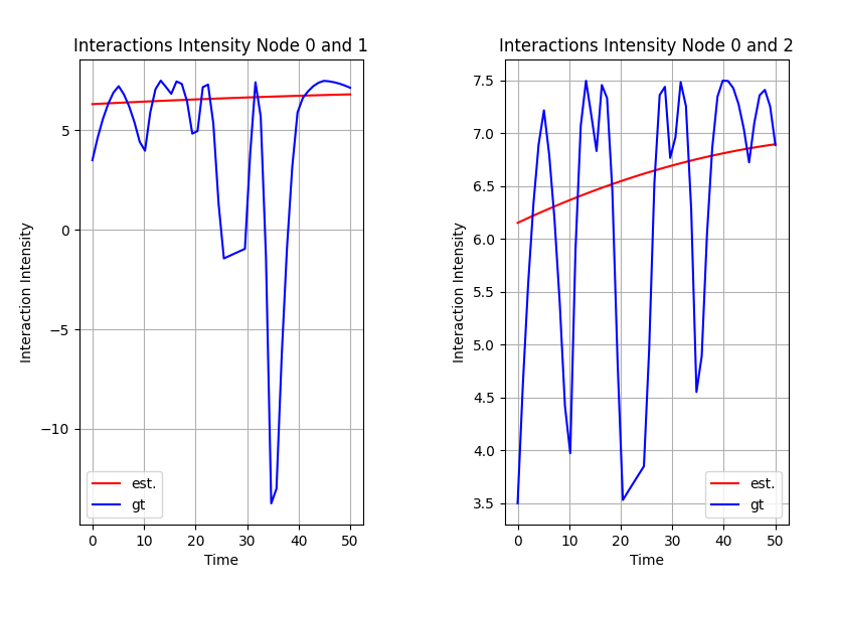
\includegraphics[width=0.7\textwidth]{0_images/rq1_2_1step_intensity_plot_node_01_02.PNG}
    \end{subfigure}
    \vfill
    \begin{subfigure}[b]{\textwidth}
        \centering
        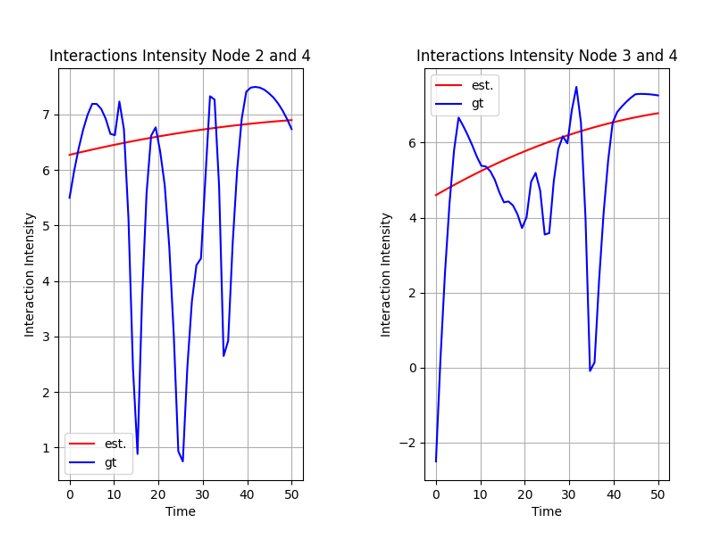
\includegraphics[width=0.7\textwidth]{0_images/rq1_2_1step_intensity_plot_node_23_34.PNG}
    \end{subfigure}
    \caption{Single step SCVM model's node pair interaction intensity for synthetic dataset 2 trained for 5000 epochs. Blue line is the ground truth model, red is the fitted model.}
    \label{fig:RQ1:part2:1step_intensity}
\end{figure}
\vspace*{-0.1cm}
\noindent
The single step SCVM is clearly limited by only fitting one step to the data, ie. having one velocity vector for each node.
For the interaction intensity plots for the remaining dyads, modelled by the single step SCVM, see appendix \ref{appendix:rq1:part2:1step_intensity}.
\\\\
The intensity rate plots, for dyad (0,1), (0,2), (2,4) and (3,4) again, as modelled by the 10 step SCVM trained for 5000 epochs, can be seen in figure \ref{fig:RQ1:part2:10step_intensity} below.
\begin{figure}[H]
    \centering
    \begin{subfigure}[b]{0.9\textwidth}
        \centering
        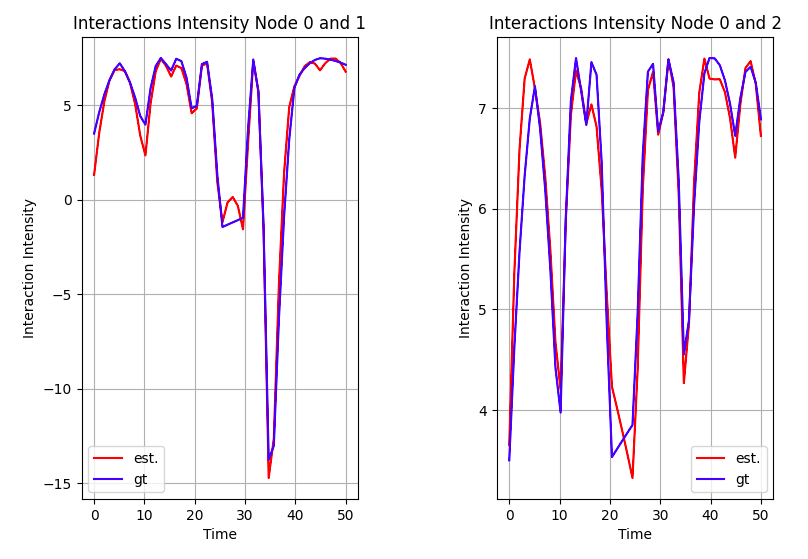
\includegraphics[width=0.8\textwidth]{0_images/rq1_10step_SCVM_intensity1.png}
    \end{subfigure}
    \vfill
    \begin{subfigure}[b]{0.45\textwidth}
        \centering
        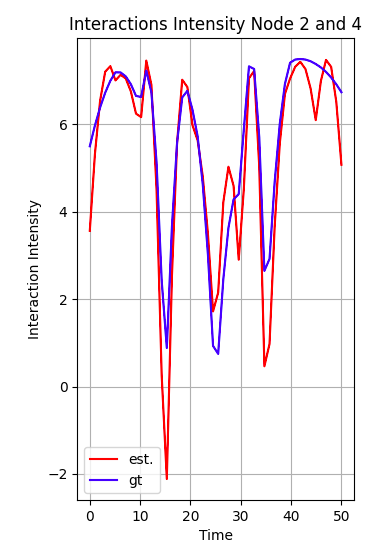
\includegraphics[width=0.8\textwidth]{0_images/rq1_10step_SCVM_intensity3.png}
    \end{subfigure}
    \hfill
    \begin{subfigure}[b]{0.45\textwidth}
        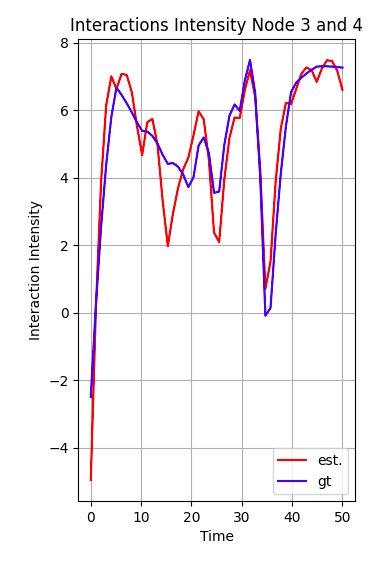
\includegraphics[width=0.8\textwidth]{0_images/rq1_10step_SCVM_intensity2.png}
    \end{subfigure}
    \caption{10 step SCVM model's node pair interaction intensities for synthetic dataset 2 trained for 5000 epochs. Blue line is the ground truth model, red is the fitted model.}
    \label{fig:RQ1:part2:10step_intensity}
\end{figure}
\noindent
The modelling capabilities of the SCVM clearly benefit from being able to fit multiple steps, ie. multiple velocity vectors for each node, in order to fit the data correctly.
All interaction intensity plots for the 10 step SCVM can be inspected in appendix \ref{appendix:rq1:part2:10step_intensity}.
\\\\
\textbf{Interaction removal results}
\\
The accuracy on removed interactions for the single step SCVM model are shown in figure \ref{fig:RQ1:1step_SCVM_accuracy} below.
\begin{figure}[H]
    \centering
    \centering
    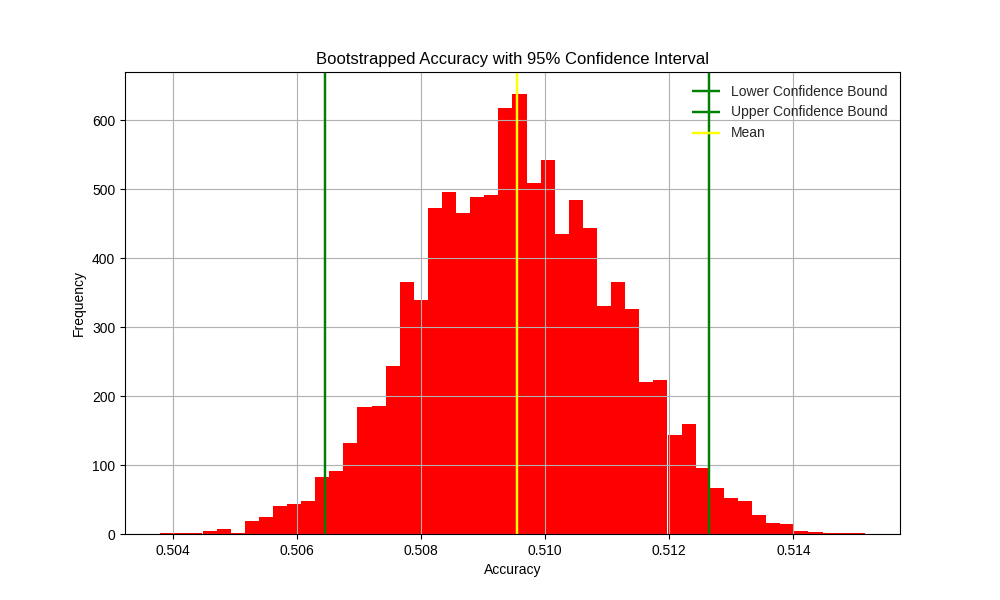
\includegraphics[width=0.8\textwidth]{0_images/rq1_2_1step_accuracy_plot.png}
    \caption{Single step SCVM model's interaction removal accuracy with 95 \% confidence inter for synthetic dataset 2 trained for 5000 epochs.}
    \label{fig:RQ1:1step_SCVM_accuracy}
\end{figure}
\noindent
The accuracy confidence interval shows an accuracy of the single step model which is little above random. 
\clearpage
\vspace*{-2cm}
\noindent
The accuracy on removed interactions for the 10 step SCVM model are seen in figure \ref{fig:RQ1:10step_SCVM_accuracy}, and the ground truth is shown in figure \ref{fig:RQ1:GT10_SCVM_accuracy}.
\begin{figure}[H]
    \centering
    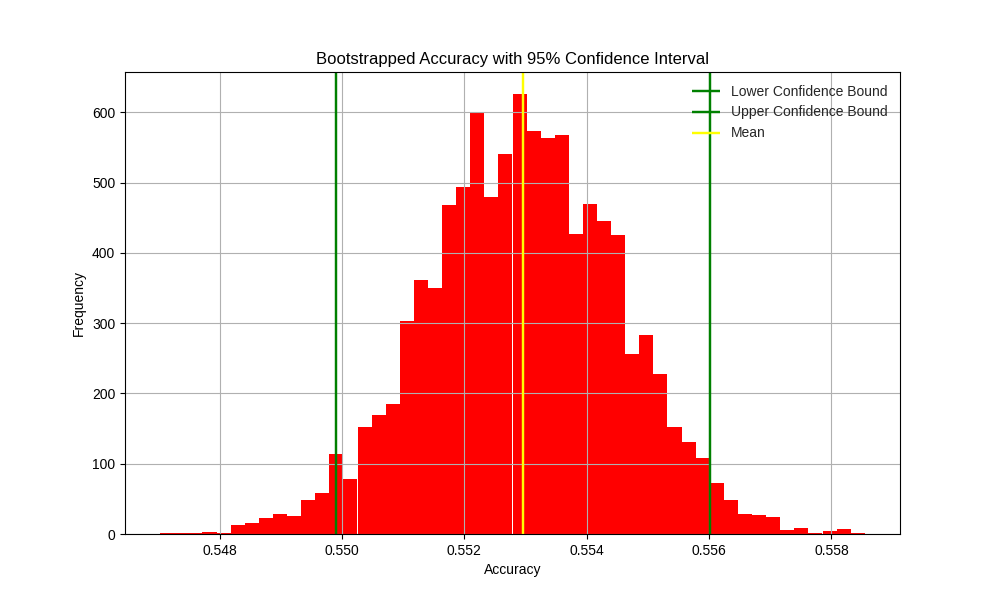
\includegraphics[width=0.8\textwidth]{0_images/10step_SCVM_Accuracy_Plot.png}
    \caption{10 step SCVM model's interaction removal accuracy with 95 \% confidence interval for synthetic dataset 2 trained for 5000 epochs.}
    \label{fig:RQ1:10step_SCVM_accuracy}
\end{figure}
\begin{figure}[H]
    \centering
    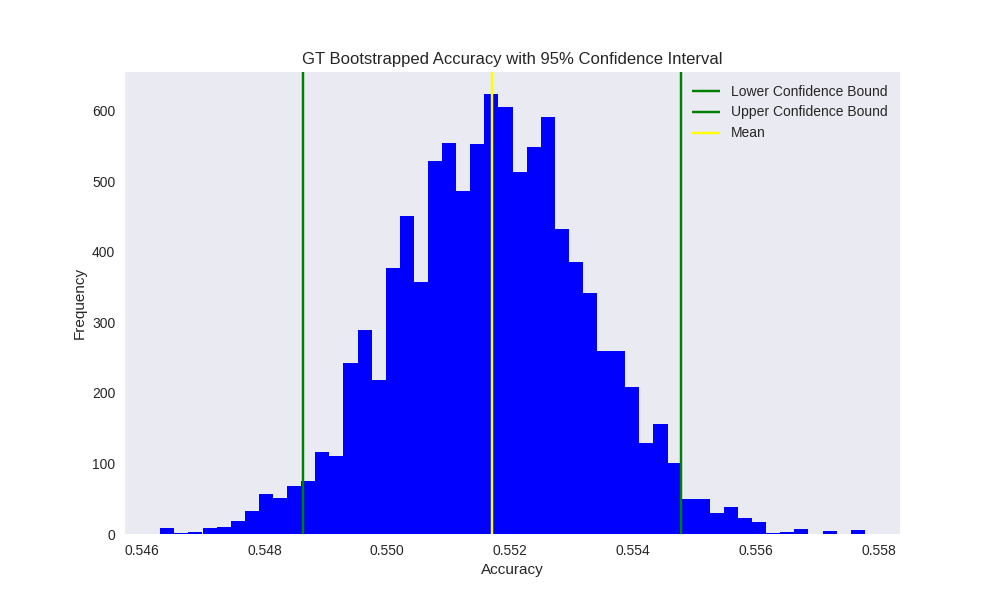
\includegraphics[width=0.8\textwidth]{0_images/10step_SCVM_GT_Accuracy_Plot.png}
    \caption{Ground truth interaction removal accuracy 95 \% confidence interval for synthetic dataset 2}
    \label{fig:RQ1:GT10_SCVM_accuracy}
\end{figure}
\noindent
Here, we also see an accuracy close to random for the 10 step SCVM, yet higher than that of the one step. 
However, the accuracy of the model matches that of the ground truth, which also only achieves around 55 \% accuracy on the synthetic dataset 2.
\clearpage
\vspace*{-2cm}
\noindent
\textbf{Dyad removal results}
\\
The interaction intensity plots after removing dyad (0,2) for the single step SCVM were just as bad as for the initial fits, where no dyads were removed, with the difference being that intensities for the removed dyad are overall lower.
This speaks of the limitation the single step modelling approach has when fitting data with stepwise dynamics. 
All interaction intensity plots for the single step SCVM after removal of node dyad (0,2) are seen, in appendix \ref{appendix:rq1:part2:1step_dyad_remove}.
\\\\
The dyad removal results for the 10 step SCVM are shown in figure \ref{fig:RQ1:10step_SCVM_dyadremoval}:
\begin{figure}[H]
    \centering
    \begin{subfigure}[b]{\textwidth}
        \centering
        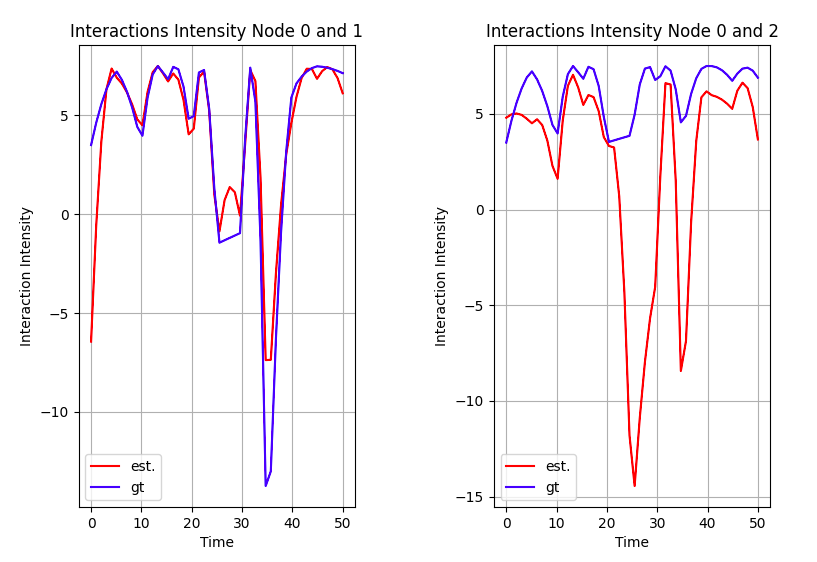
\includegraphics[width=0.7\textwidth]{0_images/10step_SCVM_dyad_removal_plot1.png}
    \end{subfigure}
    \hfill
    \begin{subfigure}[b]{\textwidth}
        \centering
        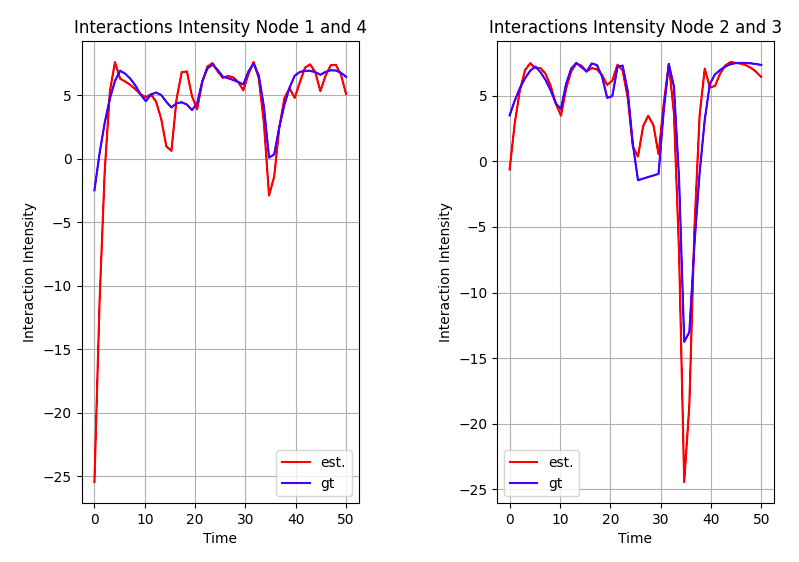
\includegraphics[width=0.7\textwidth]{0_images/10step_SCVM_dyad_removal_plot2.png}
    \end{subfigure}
        \caption{10 step SCVM intensity plot after removing node pair (0,2)}
    \label{fig:RQ1:10step_SCVM_dyadremoval}
\end{figure}
\noindent
Here, the 10 step SCVM does not have too much trouble fitting the kept node pairs, but it still struggles with parts of the intensity for the removed dyad (0,2). 
For all interaction intensity plots of the dyad removal for 10 step SCVM, see appendix \ref{appendix:rq1:part2:10step_dyad_remove}.


\subsubsection{Multi-step modelling of real world data}
\label{sec:ResearchQuestion1:ResistanceTraining}
The third part of answering the first research question investigates the SCVM's modelling capabilities on a real world dataset using 100 velocity steps. 
The dataset used for testing is the real dataset 1, the resistance game, presented in section \ref{sec:Data:RealData:RealDataset1}.
\\\\
\textbf{Interaction removal results}
\\
Since the dataset has ground truth parameters, as with the synthetic data the 100 step SCVM is evaluated using the interaction removal test, seen in figure \ref{fig:RQ1:real_SCVM_accuracy}.
\begin{figure}[H]
    \centering
    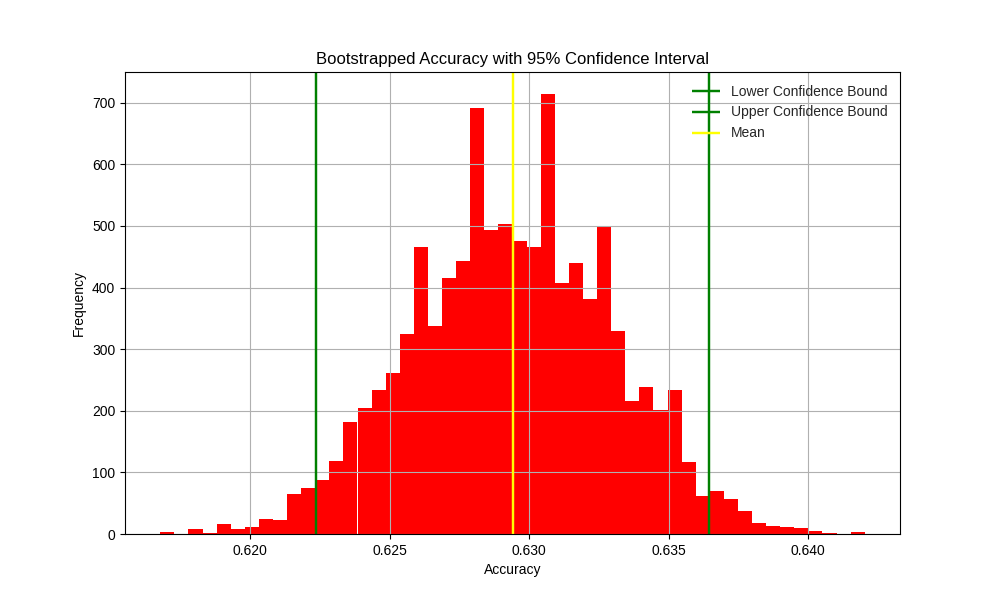
\includegraphics[width=\textwidth]{0_images/100steps_SCVM_real_dataset_accuracy_plot.png}
    \caption{100 step SCVM model's interaction removal accuracy 95 \% confidence for real dataset 1 trained for 5000 epochs.}
    \label{fig:RQ1:real_SCVM_accuracy}
\end{figure}
\noindent
For the real dataset 1, the SCVM model achieves an accuracy score of around 63 \%, which is higher than the random baseline of 50 \%, as well as the accuracy results from tests on the synthetic datasets.